\chapter{System Evaluation}
This chapter presents the evaluation of the system infrastructure, architecture and the verification and validation techniques used. Also results from the machine 
learning models were presented and analyzed. 


\section{System Verification}
Several components of the system interact together to perform the functionalities of the system and thus it is important to verify that each component works as 
expected. Each component was tested as a separate unit employing a test-driven development approach. An automated test suites were written for every functional component
of the system to test its correctness and reliability.
\subsection{Unit Testing}
An automated unit testing strategy was employed to verify continuously evolving components of the system. This strategy was also utilized for Regression Testing
to detect any breaking changes that may be introduced by new codes.
User's data were derived from different collections (Biometric data \& Performance data) of the Firestore database and were combined together as a single tuple in the 
relational database.  The testing effort was focused on boiler-plate CRUD (Create, Read, Update, Delete) required to synchronize data between the databases and service 
the various API endpoints. Test cases for Asynchronous Javascript and XML (AJAX) calls were written to verify the integrity of data being fetched from the API endpoints. 
Unit tests suites were developed using Mocha for both the Dashboard and Controller components. Fig~\ref{image:test_cases} shows the test cases developed for the 
system. 

\begin{figure}[H]
    \centering
    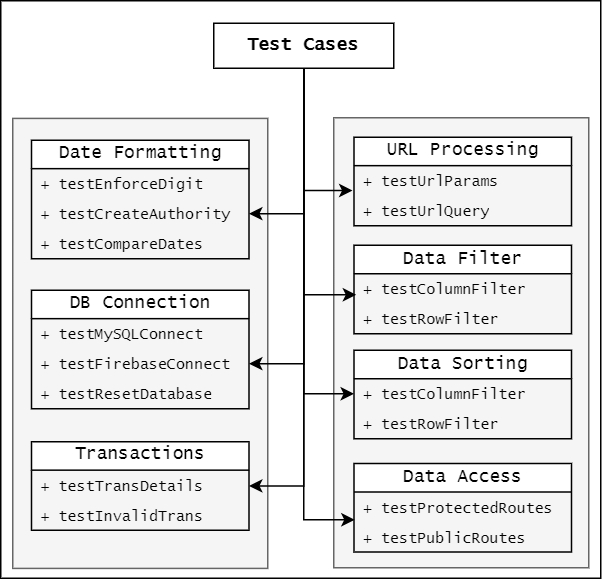
\includegraphics[width=0.8\textwidth]{images/test_cases.png}
    \caption{Test Cases}
    \label{image:test_cases}
\end{figure}

\section{System Validation}

Validating the system involves ensuring that the system meets the stated requirements and objectives. Acceptance testing was carried out to verify that the 
proposed functionalities of the system were implemented satisfactorily. The Acceptance testing was carried out with real data with the help of the supervising
lecturer and volunteers. Functional and non-functional testing was carried out to validate the system requirements, performance, and security. 
The following metrics were used to validate the system: 
\begin{itemize}
    \item \textbf{Performance} - The system was tested for handling multiple requests by simulating multiple users using Postman to send requests. The system satisfactorily
    serviced all requests without any noticeable delay. 
    \item \textbf{Security} - The system was tested for security by attempting to access the API endpoints without the required authentication. Such requests were rejected
    and appropriate error messages and code were returned. 
    \item \textbf{Accessibility} - The system was tested for accessibility using different devices and browsers to ensure a consistent user experience across board and
    validate that AJAX calls were handled correctly across different browser implementations. 
    \item \textbf{Usability} - The system was tested for usability, as the system was designed for non-technical users with the help of volunteers. The User
    Interface were supposed to be minimalistic and provide all functionalities in a single view. The users were able to perform the required tasks without any assistance.
\end{itemize}

\section{Machine Learning Model Evaluation}

\subsubsection{Actual vs Predicted Analysis}
The actual values were plotted against the predicted values to see how well the model predicted the
dependent variables. The plot was used to see if the model was underfitting or overfitting the data. If the points were close to the line, it indicated that the model was performing well.
If the points were scattered, it indicated that the model was not performing well. It was also used to see if the model was capturing the underlying patterns in the data. Below are the
actual versus predicted plots for the best-performing model for each dependent variable.

\subsection*{Fine Motor Tracking Time}

\begin{figure}[htbp]
    \centering
    \begin{subfigure}[b]{0.49\textwidth}
        \centering
        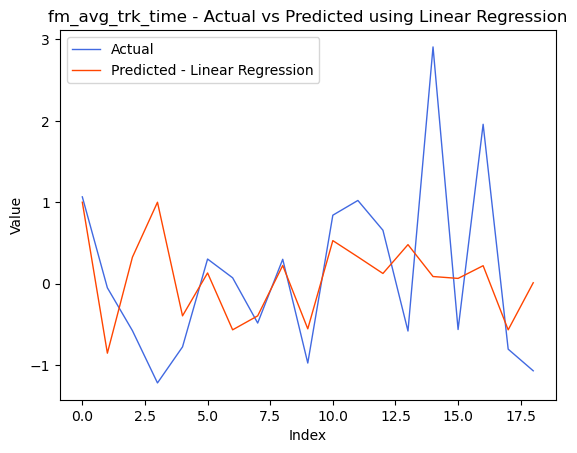
\includegraphics[width=\textwidth]{images/regressionCharts/test_data_fine_motor_tracking_time.png}
        \caption{Actual vs Predicted (Test Data)}
        \label{fig:actual_vs_predicted_fm_avg_trk_time_test}
    \end{subfigure}\hfill
    \begin{subfigure}[b]{0.49\textwidth}
        \centering
        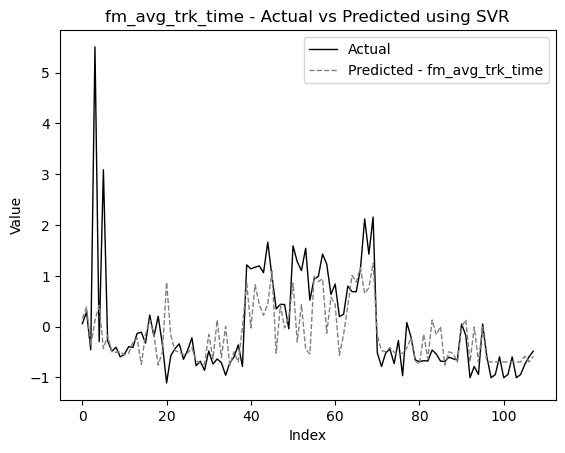
\includegraphics[width=\textwidth]{images/regressionCharts/all_data_fine_motor_tracking_time.png}
        \caption{Actual vs Predicted (All Data)}
        \label{fig:actual_vs_predicted_fm_avg_trk_time_all_data}
    \end{subfigure}
    \caption{Fine Motor Tracking Time Actual vs Predicted}
    \label{fig:fine_motor_tracking_time_comparison}
\end{figure}

\subsubsection*{Test Data Evaluation}

\begin{itemize}
    \item \textbf{Trend}: Figure \ref{fig:actual_vs_predicted_fm_avg_trk_time_test} shows the actual versus predicted values for the Fine Motor Average Tracking Time using the test data. The model that performed
          the best for this dependent variable was the Support Vector Regressor. The predictions generally matched the trajectory of the actual test data. The peaks and troughs of the
          actual data were also found in the predicted data, with some deviations.
    \item \textbf{Variance}: There is a noticeable variance between the actual and predicted values, especially at the extremes. For instance, the model appears to underestimate the highest values
          and overestimate the lowest values.
    \item \textbf{Consistency}: The model shows decent consistency when the actual values are around the mean but is less consistent at capturing sudden changes in the actual data, such as sharp spikes ot dips.
\end{itemize}

\subsubsection*{All Data Evaluation}

\begin{itemize}
    \item \textbf{Trend}: Figure \ref{fig:actual_vs_predicted_fm_avg_trk_time_all_data} shows the actual versus predicted values for the Fine Motor Average Tracking Time using all the data
          available. When evaluating all the data, the model predictions closely follow the actual data's trend. This indicates that the model has learned the overall behavior of the dataset quite well.
          Similar to the test data, the model captures the general pattern of movement in the actual values, but might not always match the amplitude of changes.
    \item \textbf{Variance}: The variance between the actual and predicted values over all the data seems to be lower compared to the test data. This suggests that the model has been
          effectively trained to understand the data as a whole. Some exceptions occur where the actual values show significant deviation from the mean. In these areas, the predictions do not fully
          capture the extent of the actual values and show some deviation.
    \item \textbf{Consistency}: The model shows good consistency in predicting the values when the actual values are around the mean. The predictions often match the actual values quite closely.
\end{itemize}

Overall the Support Vector Regressor Model performed well in both scenarios, capturing the general trends of the Fine Motor Tracking Time and showing good consistency in prediction.
The model, however, seems to struggle with accurately predicting the more extreme values in the dataset. It highlights the need for improving the model's performance on the more complex
or extreme segments of the data.

\subsection*{Fine Motor Accuracy}

\begin{figure}[htbp]
    \centering
    \begin{subfigure}[b]{0.49\textwidth}
        \centering
        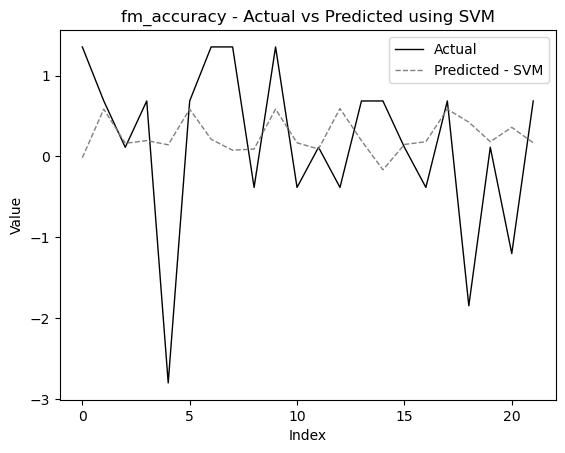
\includegraphics[width=\textwidth]{images/regressionCharts/test_data_fine_motor_accuracy.png}
        \caption{Actual vs Predicted (Test Data)}
        \label{fig:actual_vs_predicted_fm_accuracy_test}
    \end{subfigure}\hfill
    \begin{subfigure}[b]{0.49\textwidth}
        \centering
        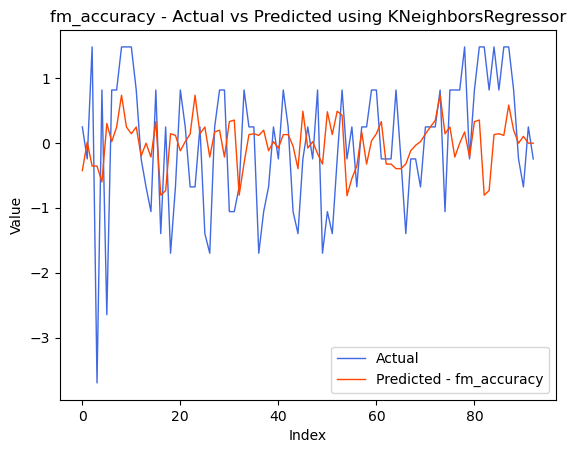
\includegraphics[width=\textwidth]{images/regressionCharts/all_data_fine_motor_accuracy.png}
        \caption{Actual vs Predicted (All Data)}
        \label{fig:actual_vs_predicted_fm_accuracy_all_data}
    \end{subfigure}
    \caption{Fine Motor Accuracy Actual vs Predicted}
    \label{fig:fine_motor_accuracy_comparison}
\end{figure}

\subsubsection*{Test Data Evaluation}

\begin{itemize}
    \item \textbf{Trend}: Figure \ref{fig:actual_vs_predicted_fm_accuracy_test} shows the actual versus predicted values for the Fine Motor Accuracy using the test data. The model
          that performed the best for this dependent variable was the Support Vector Regressor. The model appears to capture the general trend of the actual data. It follows the directional
          changes, going up and down as the actual values do, but not with perfect alignment.
    \item \textbf{Variance}: A noticeable discrepancy between the actual and predicted values is noted, particularly evident at the extremes. While the model tends to underpredict some of the sharper
          declines in actual values, it remains relatively close to the true data points.
    \item \textbf{Consistency}: There is a moderate level of consistency in the predictions. The model seems to perform well when the actual values are not showing extreme behavior. However,
          in instances where the actual values show sharp changes, the model's consistency is reduced.
\end{itemize}

\subsubsection*{All Data Evaluation}

\begin{itemize}
    \item \textbf{Trend}: Figure \ref{fig:actual_vs_predicted_fm_accuracy_all_data} shows the actual versus predicted values for the Fine Motor Accuracy using all the data available.
          Across the full dataset, the Support Vector Regressor model generally traces the movements of the actual values well. This suggests a solid understanding of the underlying patterns
          in the full range of data. Despite some misalignment, the predicted values consistently mirror the ups and downs in the actual data, indicating the model's capability to track the
          overall trend.
    \item \textbf{Variance}: Compared to the test data, the variance in the full data set appears to be slightly more visible. The predictions occasionally deviate significantly from the
          actual values, particularly where there are sharp changes in the actual data or outliers in the actual data.
    \item \textbf{Consistency}: The model shows good consistency in predicting the values when the actual values are around the mean. It does, however, display some inconsistencies, again
          mainly where there are larger deviations in the actual data.
\end{itemize}

Overall, the Support Vector Regressor model demonstrated an ability to find the overall patterns in the Fine Motor Accuracy, both in the test set and the full dataset. While the model tends
to stay close to the actual values, it does show some variance and inconsistency, particularly in areas where the actual data shows sharp changes or outliers. This suggests that the
model may need further refinement to improve its performance in these more complex or extreme segments of the data. Also, the model may benefit from more data to help it better understand
the full range of patterns in the dataset.

\subsection*{Visual Average Response Time}

\begin{figure}[htbp]
    \centering
    \begin{subfigure}[b]{0.49\textwidth}
        \centering
        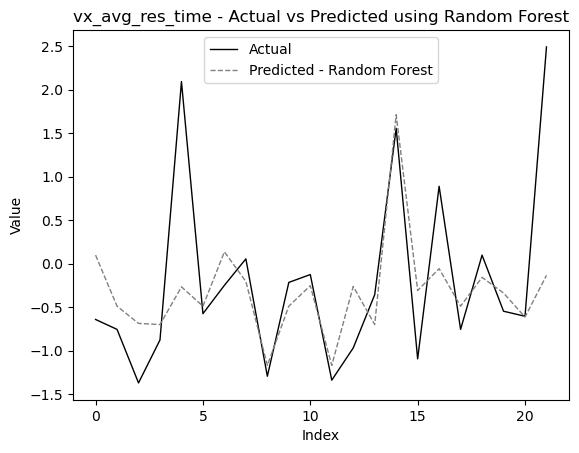
\includegraphics[width=\textwidth]{images/regressionCharts/test_data_visual_average_response_time.png}
        \caption{Actual vs Predicted (Test Data)}
        \label{fig:actual_vs_predicted_vx_avg_res_time_test}
    \end{subfigure}\hfill
    \begin{subfigure}[b]{0.49\textwidth}
        \centering
        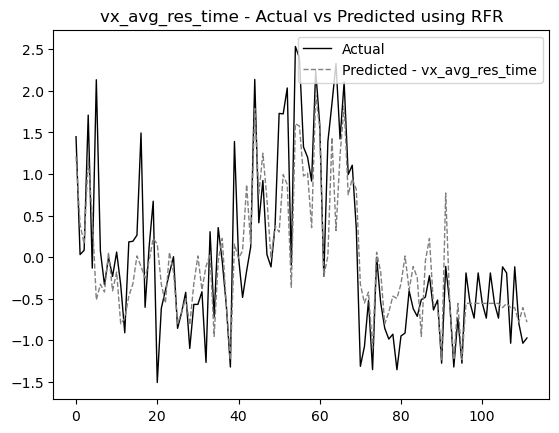
\includegraphics[width=\textwidth]{images/regressionCharts/all_data_visual_average_response_time.png}
        \caption{Actual vs Predicted (All Data)}
        \label{fig:actual_vs_predicted_vx_avg_res_time_all_data}
    \end{subfigure}
    \caption{Visual Average Response Time Actual vs Predicted}
    \label{fig:visual_avg_response_time_comparison}
\end{figure}

\subsubsection*{Test Data Evaluation}

\begin{itemize}
    \item \textbf{Trend}: Figure \ref{fig:actual_vs_predicted_vx_avg_res_time_test} shows the actual versus predicted values for the Visual Average Response Time using the test data.
        The model that performed the best for this dependent variable was the Random Forest Regressor. The model successfully captured the underlying trend of the actual data. 
        It demonstrates an ability to learn the fundamental patterns in the data, following the general trajectory of the actual values.
    \item \textbf{Variance}: While the model generally aligns with the actual values, there are areas where the deviation from the actual data is noticeable. The model doesn't
          always capture the sharpness and valleys which can be seen in several areas of the actual data.
    \item \textbf{Consistency}: In sections where the data does not fluctuate significantly, the predictions are consistent with the actual values. This suggests a level
          of reliability of the model, under the condition that the actual data does not show extreme behavior. 
\end{itemize}

\subsubsection*{All Data Evaluation}

\begin{itemize}
    \item \textbf{Trend}: Figure \ref{fig:actual_vs_predicted_vx_avg_res_time_all_data} shows the actual versus predicted values for the Visual Average Response Time using all the data available.
          When applied to the entire dataset, the model displays an ability to mimic the overall trend line of the actual data. The predictions fluctuate in line with the actual values,
          showing an understanding of the larger patterns in the data.
    \item \textbf{Variance}: As with the test data, there are discrepancies between the actual and predicted values; these are most apparent where there is a sharp change in the actual data.
          The model sometimes smooths out these abrupt changes, leading to a slight deviation from the actual values.
    \item \textbf{Consistency}: The model shows a decent level of consistency throughout the entire data range. While there are mismatches, particularly in areas of high variability,
          the model maintains a close following with the actual values for the most part.
\end{itemize}

In both the test data and the full dataset, the Random Forest Regressor model for the Visual Average Response Time demonstrates effectiveness in capturing the main trends and movements.
It shows a good degree of consistency, with understandable variance in places where the data is more complex or extreme. The model appears to perform better when dealing with average levels of
fluctuation but might require further tuning to more accurately predict the more extreme variations observed in the actual data.


\subsection*{Visual Shot Accuracy}

\begin{figure}[htbp]
    \centering
    \begin{subfigure}[b]{0.49\textwidth}
        \centering
        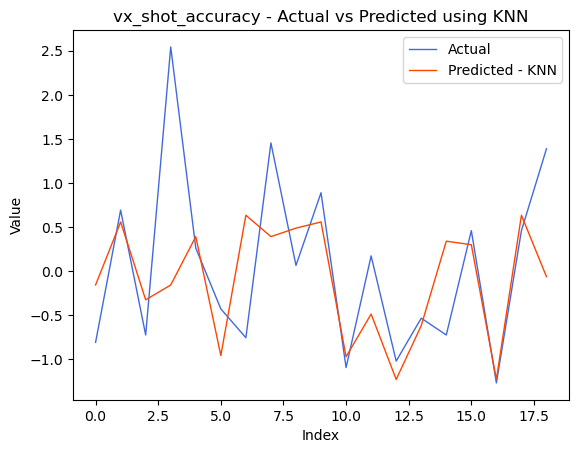
\includegraphics[width=\textwidth]{images/regressionCharts/test_data_visual_shot_accuracy.png}
        \caption{Actual vs Predicted (Test Data)}
        \label{fig:actual_vs_predicted_vx_shot_accuracy_test}
    \end{subfigure}\hfill
    \begin{subfigure}[b]{0.49\textwidth}
        \centering
        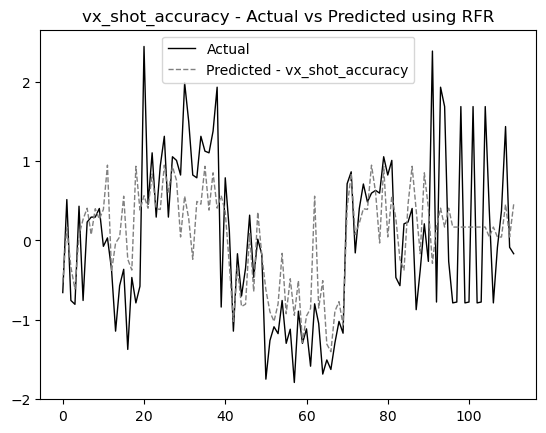
\includegraphics[width=\textwidth]{images/regressionCharts/all_data_visual_shot_accuracy.png}
        \caption{Actual vs Predicted (All Data)}
        \label{fig:actual_vs_predicted_vx_shot_accuracy_all_data}
    \end{subfigure}
    \caption{Visual Shot Accuracy Actual vs Predicted}
    \label{fig:visual_shot_accuracy_comparison}
\end{figure}

\subsubsection*{Test Data Evaluation}

\begin{itemize}
    \item \textbf{Trend}: Figure \ref{fig:actual_vs_predicted_vx_shot_accuracy_test} shows the actual versus predicted values for the Visual Shot Accuracy using the test data. The model that performed
          the best for this dependent variable was the Random Forest Regressor. The model seems to reasonably follow the general of the actual values. It responds to the directional shifts in the data,
          rising and falling in correlation with the actual data. However, there are noticeable disparities at certain points, indicating that while the model detects the overall pattern, it does not always align
          perfectly with the actual data's trajectory.
    \item \textbf{Variance}: It is clear that the model's predictions do not perfectly match the actual values, especially at the peaks. The model performs
          more reliably at data points that are closer to the central trend and show more deviation at the extremes.
    \item \textbf{Consistency}: The model demonstrates moderate consistency throughout the test dataset, capturing the general trend of the actual data with some fidelity. However, \\
          its ability to mirror the actual data precisely at every point is limited, especially where there is significant fluctuation in the actual data.

\end{itemize}

\subsubsection*{All Data Evaluation}

\begin{itemize}
    \item \textbf{Trend}: Figure \ref{fig:actual_vs_predicted_vx_shot_accuracy_all_data} shows the actual versus predicted values for the Visual Shot Accuracy using all the data available.
          With the entire dataset, the model's prediction still follows the actual values' general trend, suggesting an understanding of the global behavior of the data. The model struggles
          with sharp spikes and drops, smoothing over some of the more extreme changes in the actual data.

    \item \textbf{Variance}: The variance across the full dataset seems to be slightly more controlled than in the test data, although discrepancies remain. The model does not perfectly capture
          the amplitude of changes, particularly the higher peaks and lower troughs in the actual data.

    \item \textbf{Consistency}: Across the full scope of data, the model's predictions display an adequate level of consistency, reflecting a steady predictive performance that often aligns well with the real values.
          However, the model's prediction can diverge from the actual data at points, indicating room for improvement in model accuracy.

\end{itemize}

The Random Forest Regressor model shows that it captured the central tendencies and fluctuations in Visual Shot Accuracy both in the testing phase and across the complete dataset. The model's capability of
following the trends is a strong point, but its prediction variance and the consistency of its performance present areas for improvement.


\subsection*{Visual Target Accuracy}

\begin{figure}[htbp]
    \centering
    \begin{subfigure}[b]{0.49\textwidth}
        \centering
        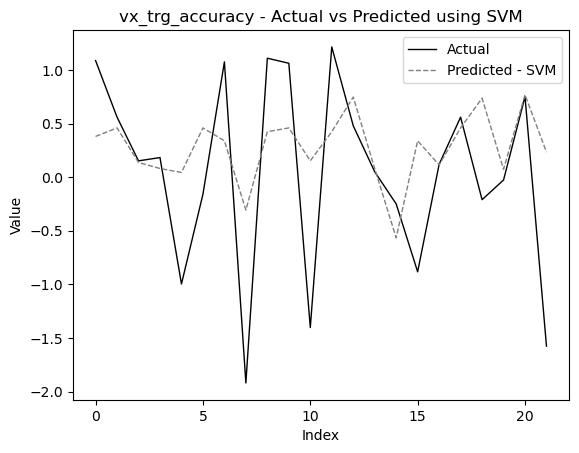
\includegraphics[width=\textwidth]{images/regressionCharts/test_data_visual_target_accuracy.png}
        \caption{Actual vs Predicted (Test Data)}
        \label{fig:actual_vs_predicted_vx_trg_accuracy_test}
    \end{subfigure}\hfill
    \begin{subfigure}[b]{0.49\textwidth}
        \centering
        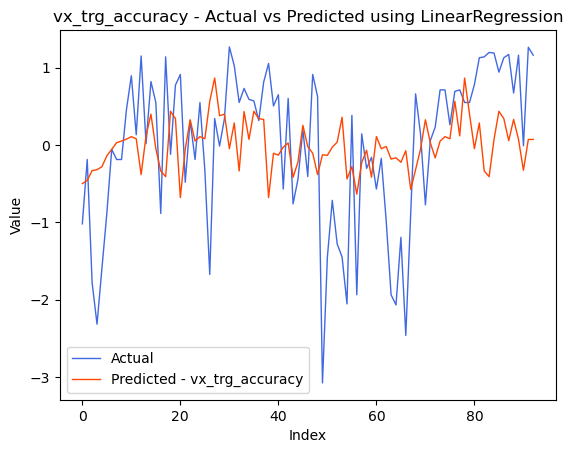
\includegraphics[width=\textwidth]{images/regressionCharts/all_data_visual_target_accuracy.png}
        \caption{Actual vs Predicted (All Data)}
        \label{fig:actual_vs_predicted_vx_trg_accuracy_all_data}
    \end{subfigure}
    \caption{Visual Target Accuracy Actual vs Predicted}
    \label{fig:visual_target_accuracy_comparison}
\end{figure}

\subsubsection*{Test Data Evaluation}

\begin{itemize}
    \item \textbf{Trend}: Figure \ref{fig:actual_vs_predicted_vx_trg_accuracy_test} shows the actual versus predicted values for the Visual Target Accuracy using the test data. The model that performed
          best for this dependent variable was the Support Vector Regressor Model. The model's predicted outcomes show a basic alignment with the actual data's trend. The general ups and downs in the actual data are
          mirrored in the model's predictions, indicating a broad understanding of the data's patterns. However, there are instances where the model does not perfectly trace the actual data's peaks and troughs,
          suggesting that while the trend is recognized, the precision of the model could be improved.

    \item \textbf{Variance}: The variance between the actual and predicted values seems moderate. The model seems to smooth out some of the actual data fluctuations, not capturing the extremes as it should.

    \item \textbf{Consistency}: There is a moderate level of consistency in the model's predictions across the test dataset. The predicted values are regularly close to the actual data, but 
            there are instances where the model's predictions deviate from the actual data. 
\end{itemize}

\subsubsection*{All Data Evaluation}

\begin{itemize}
    \item \textbf{Trend}: Figure \ref{fig:actual_vs_predicted_vx_trg_accuracy_all_data} shows the actual versus predicted values for the Visual Target Accuracy using all the data available. Over the entire dataset,
          the Support Vector Regressor model's predictions generally follow the trend of the actual values, indicating a stable understanding of the data's patterns. Similar to the test data, the predictions are in line with the
          overall movements but occasionally miss the mark in capturing the specific oscillations in the actual data.

    \item \textbf{Variance}: The prediction variance across the full dataset appears somewhat greater compared to the test data. This could be due to the inclusion of more diverse data points, revealing the model's
          limitations in adapting to broader patterns. The model especially tends to underpredict some of the lower values, leading to a noticeable deviation in the more extreme data points.

    \item \textbf{Consistency}: Throughout the full dataset, the consistency of the predictions are apparent but not without error. It seems to stay true to the mean trajectory but lacks in tracking the
          finer details of the actual data.

\end{itemize}

The Support Vector Regressor Model for the Visual Target Accuracy demonstrates a basic understanding of the data's patterns, capturing the general trends in the test data and the full dataset. However, the model exhibits
a level of variance that indicates room for improvement in its predictive accuracy. Specifically, the model could benefit from refinement to better capture the more extreme values in the actual data.

\subsection*{Audio Average Response Time}

\begin{figure}[htbp]
    \centering
    \begin{subfigure}[b]{0.49\textwidth}
        \centering
        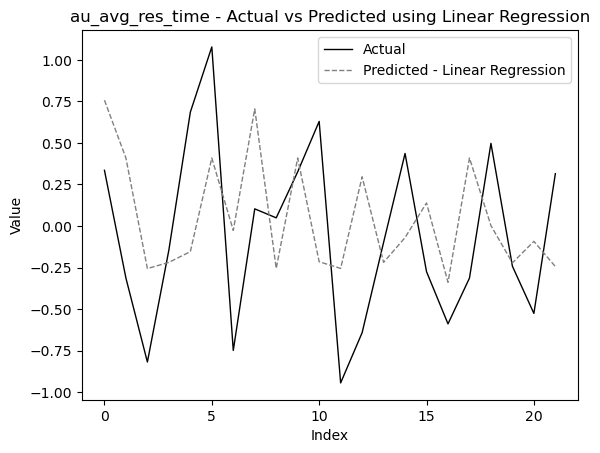
\includegraphics[width=\textwidth]{images/regressionCharts/test_data_audio_average_response_time.png}
        \caption{Actual vs Predicted (Test Data)}
        \label{fig:actual_vs_predicted_au_avg_res_time_test}
    \end{subfigure}\hfill
    \begin{subfigure}[b]{0.49\textwidth}
        \centering
        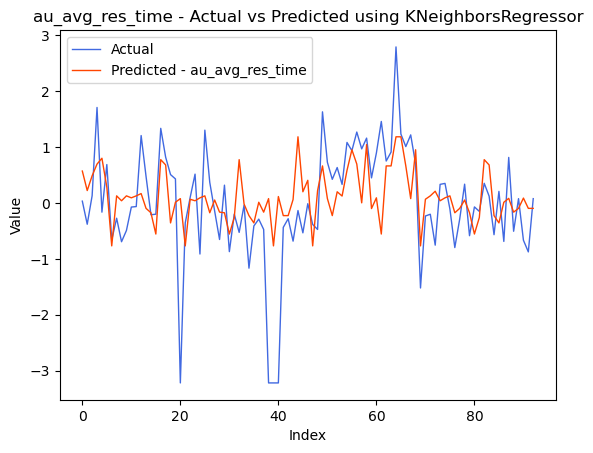
\includegraphics[width=\textwidth]{images/regressionCharts/all_data_audio_average_response_time.png}
        \caption{Actual vs Predicted (All Data)}
        \label{fig:actual_vs_predicted_au_avg_res_time_all_data}
    \end{subfigure}
    \caption{Audio Average Response Time Actual vs Predicted}
    \label{fig:audio_avg_response_time_comparison}
\end{figure}

\subsubsection*{Test Data Evaluation}

\begin{itemize}
    \item \textbf{Trend}: Figure \ref{fig:actual_vs_predicted_au_avg_res_time_test} shows the actual versus predicted values for the Audio Average Response Time using the test data. The model that performed
          best for this dependent variable was the Linear Regression. The model's predictions tend to reflect the actual data's trend, indicating a general grasp of the data's patterns. The prediction line shows
          a consistent rise and fall pattern that corresponds with the actual data line, illustrating the model's ability to track changes in response time.

    \item \textbf{Variance}: There is a significant difference between the predicted and actual values at multiple points. This difference highlights areas where the model's predictions 
            are not as close to the actual values, especially at sharp downward and upward turns in the actual data.

    \item \textbf{Consistency}: Despite some variances, the Linear Regression model remains fairly consistent in its predictions throughout the test dataset. While it does not precisely match the actual values, it provides
          a reasonably consistent estimation, particularly in the middle range of the response time values.

\end{itemize}


\subsubsection*{All Data Evaluation}

\begin{itemize}
    \item \textbf{Trend}: Figure \ref{fig:actual_vs_predicted_au_avg_res_time_all_data} shows the actual versus predicted values for the Audio Average Response Time using all the data available. Looking
          at the entire dataset, the Linear Regression model again mirrors the general trend of the actual data, showing an ability to comprehend the ups and downs in the response time. It captures the global trend across a
          broader range of data points.

    \item \textbf{Variance}: The overall variance in predictions across the entire dataset appears to be somewhat controlled, but deviations are still present. The model occasionally smoothens the extremities
          in the actual data, leading to under or overestimation in some segments.

    \item \textbf{Consistency}: In terms of consistency, the model shows a reasonable degree of reliability across the entire dataset. Its predictions are in alignment with the direction of the actual data,
          even though it does not match every peak and valley with precision.

\end{itemize}


The Linear Regression model for the Audio Average Response Time demonstrates a competent understanding of the Audio Average Response Time patterns, both in the test and the full dataset. It demonstrates
a level of consistency that suggests it captures the variable's fundamental characteristics. However, the model's prediction exhibits some variance, indicating room for improvement in its ability to capture more
subtle fluctuations in the data.



\subsection*{Model Evaluation}

The model was evaluated using the test dataset and all the data available. The predictions were compared to the actual values to assess its performance.
The actual versus predicted values were plotted to visualize how well the model predicted the dependent variables. The plots were used to compare the model's performance with the
classical machine learning models.

\begin{figure}
    \centering
    \begin{subfigure}[b]{0.49\textwidth}
        \centering
        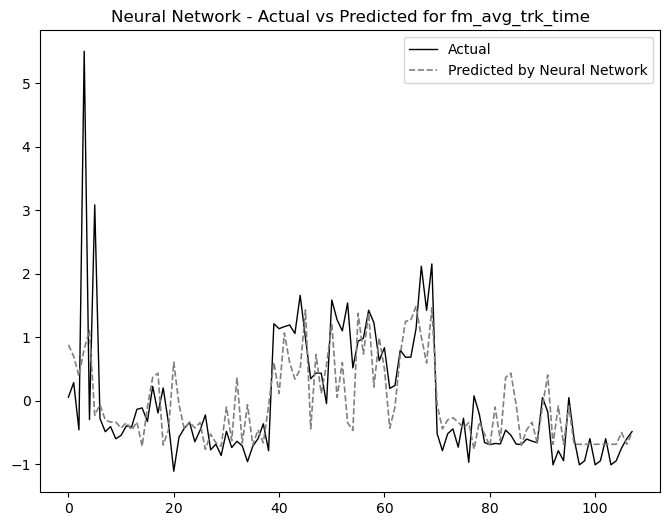
\includegraphics[width=\linewidth]{images/nnCharts/all_data_fine_motor_avg_tracking_time.png}
    \end{subfigure}\hfill
    \begin{subfigure}[b]{0.49\textwidth}
        \centering
        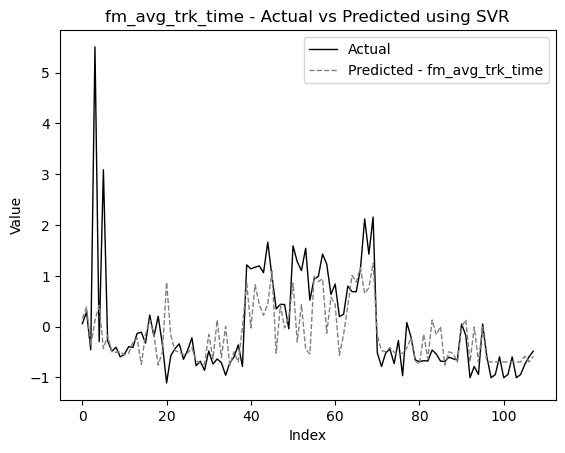
\includegraphics[width=\linewidth]{images/regressionCharts/all_data_fine_motor_tracking_time.png}
    \end{subfigure}
    
    \begin{subfigure}[b]{0.49\textwidth}
        \centering
        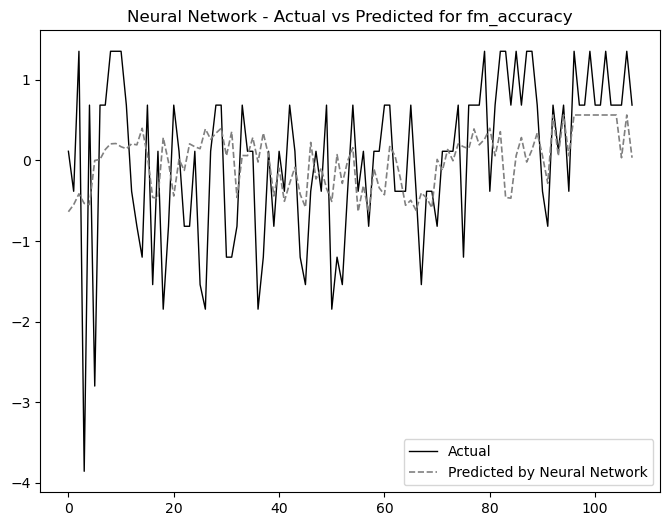
\includegraphics[width=\linewidth]{images/nnCharts/all_data_fine_motor_accuracy.png}
    \end{subfigure}\hfill
    \begin{subfigure}[b]{0.49\textwidth}
        \centering
        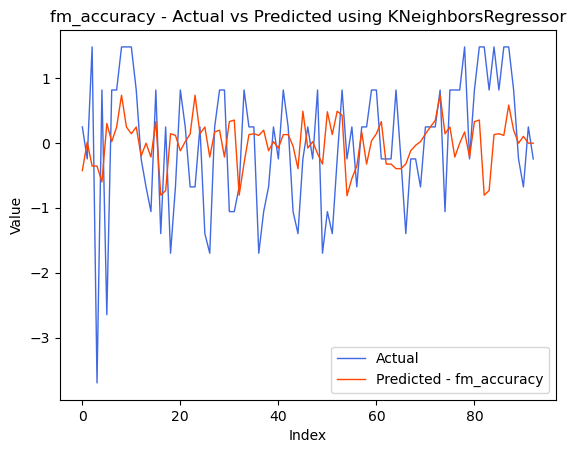
\includegraphics[width=\linewidth]{images/regressionCharts/all_data_fine_motor_accuracy.png}
    \end{subfigure}
    
    \begin{subfigure}[b]{0.49\textwidth}
        \centering
        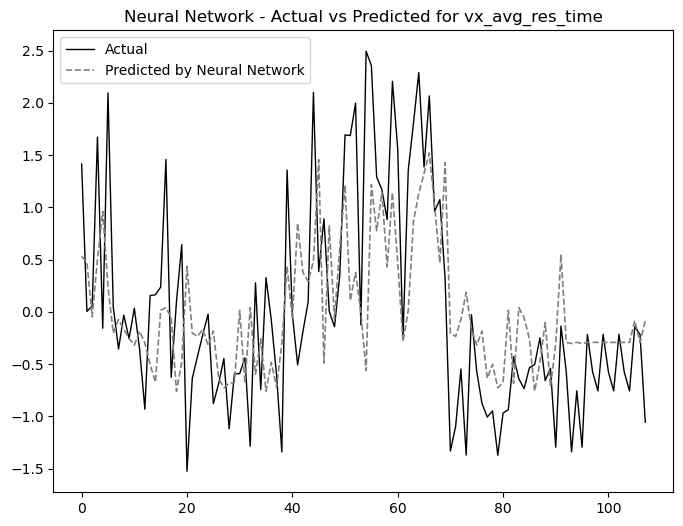
\includegraphics[width=\linewidth]{images/nnCharts/all_data_visual_avg_response_time.png}
    \end{subfigure}\hfill
    \begin{subfigure}[b]{0.49\textwidth}
        \centering
        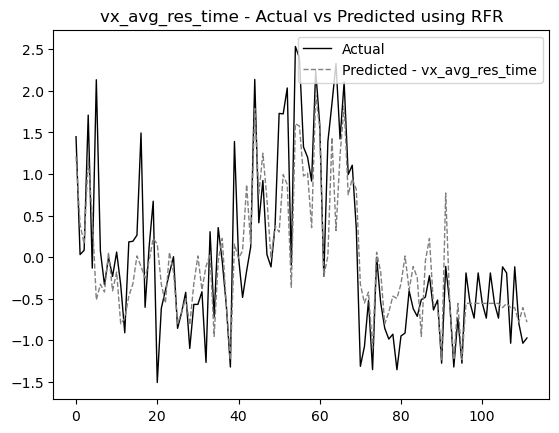
\includegraphics[width=\linewidth]{images/regressionCharts/all_data_visual_average_response_time.png}
    \end{subfigure}
    
    
    \caption{Neural Network Model vs Classical ML Models}
    \label{fig:nn_comparison}
\end{figure}



\begin{figure}
    \centering
    \begin{subfigure}[b]{0.49\textwidth}
        \centering
        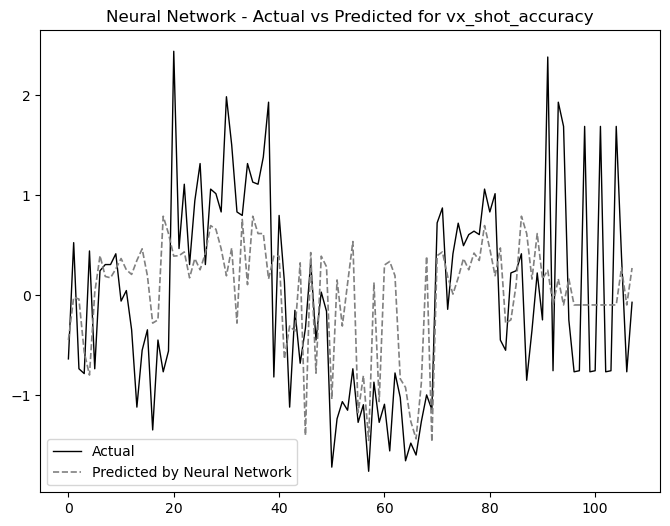
\includegraphics[width=\linewidth]{images/nnCharts/all_data_visual_shot_accuracy.png}
    \end{subfigure}\hfill
    \begin{subfigure}[b]{0.49\textwidth}
        \centering
        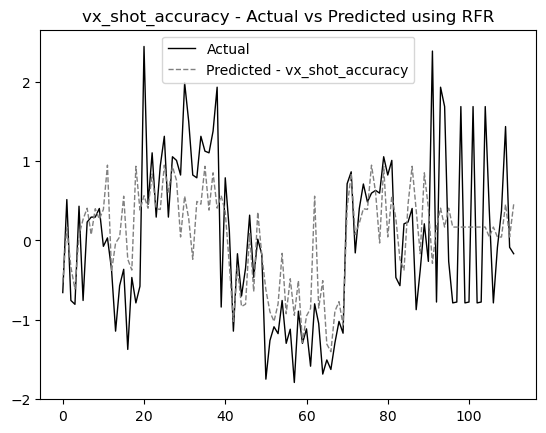
\includegraphics[width=\linewidth]{images/regressionCharts/all_data_visual_shot_accuracy.png}
    \end{subfigure}
    
    \begin{subfigure}[b]{0.49\textwidth}
        \centering
        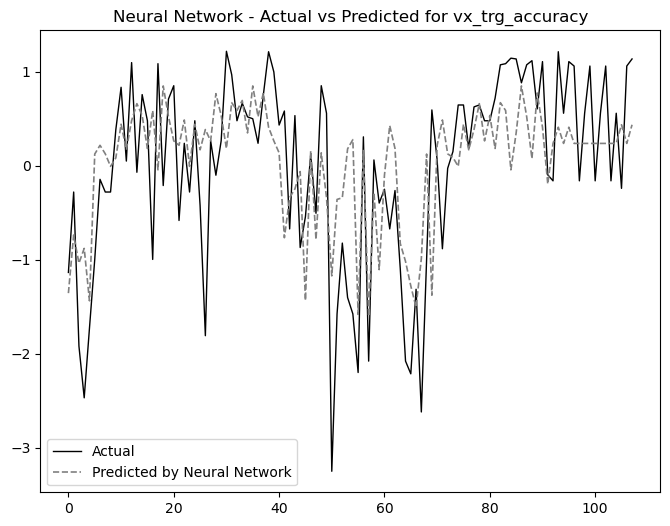
\includegraphics[width=\linewidth]{images/nnCharts/all_data_visual_target_accuracy.png}
    \end{subfigure}\hfill
    \begin{subfigure}[b]{0.49\textwidth}
        \centering
        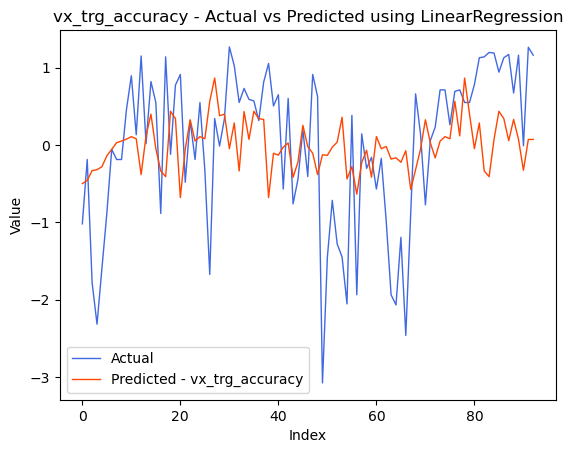
\includegraphics[width=\linewidth]{images/regressionCharts/all_data_visual_target_accuracy.png}
    \end{subfigure}
    
    \begin{subfigure}[b]{0.49\textwidth}
        \centering
        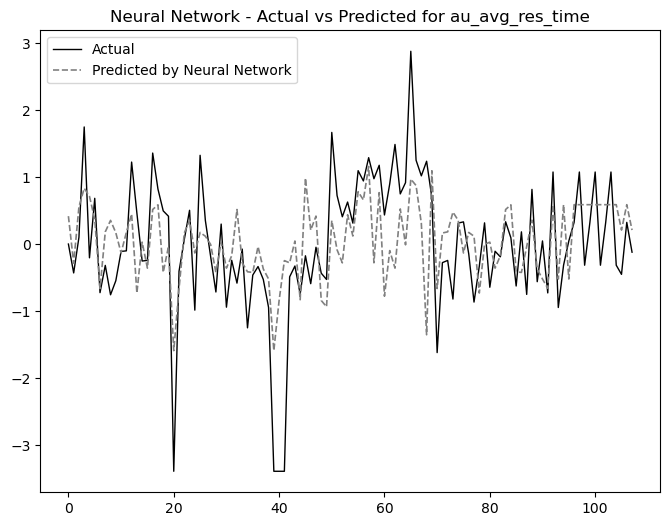
\includegraphics[width=\linewidth]{images/nnCharts/all_data_audio_avg_response_time.png}
    \end{subfigure}\hfill
    \begin{subfigure}[b]{0.49\textwidth}
        \centering
        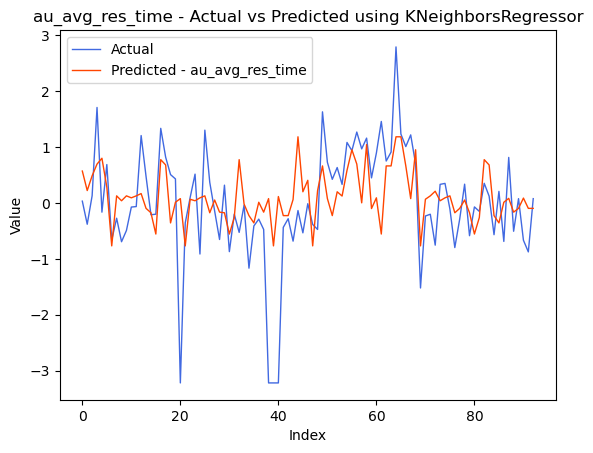
\includegraphics[width=\linewidth]{images/regressionCharts/all_data_audio_average_response_time.png}
    \end{subfigure}
    
    \caption{Neural Network Model vs Classical ML Models}
    \label{fig:nn_comparison}
\end{figure}


When contrasted with the classical machine learning models, the neural network model demonstrated an ability to capture complex, nonlinear interactions within the data, fitting closely to the 
variances and trends in the actual data. This characteristic can lead to highly accurate predictions on the training dataset but may also cause the model to overfit, as evidenced by prediction 
lines that follow the actual data with high fidelity, including noise and outliers.

\begin{itemize}
    \item \textbf{Trend}: The neural network model is dynamic, and capable of adapting to data fluctuations, which can be both an asset and a liability. They may reflect underlying patterns with precision but also amplify 
    anomalies. In contrast, classical models such as Support Vector Regressors and Random Forest Regressors favour a moderate approach, often smoothing over data to project a more stable and generalized trend line.
    
    \item \textbf{Variance}: The neural network model exhibit a higher variance in predictions compared to classical models. This can be beneficial in capturing the full range of data patterns but 
    also poses the risk of overfitting to noise and outliers. On the other hand, classical models typically show less variance, indicating a tempered response to data variability, which might overlook 
    complex patterns but also ensures robustness against noise.

    \item \textbf{Consistency}: The adaptability of neural networks, which enables them to capture a wide range of data behaviours, may also affect their consistency across different conditions.
    In contrast, the classical models can be especially valuable when the objective emphasizes stability over detailed accuracy.
    

\end{itemize}


Overall, the NN model outperforms the classical models in terms of trend following, variance capturing and overall consistency, particularly when evaluating the full dataset. This suggests that 
the neural network model is well-suited for capturing the complex relationships between the independent and dependent variables in the dataset, while classical models provide a more generalized
approach that may be more suitable for stable, less complex datasets.
For this project, due to a very close performance between the neural network and classical models, we conclude that as the dataset grows, the neural network model may be more suitable for capturing
the complex relationships between the independent and dependent variables in the dataset, but the classical models should not be overlooked as they provide a more generalized approach that may
be more suitable for stable, less complex datasets.

The balance between sensitivity to data changes and maintaining a level of generalization seems to be the area where the neural network's performance could be further optimized.

\section{Project Objectives}
The initial project objective was to build an enduring infrastructure that can access user's data and do real-time analysis. The system was shown to be able to reliably 
perform the stated tasks effectively. The achievement recorded in this project is summarized below:
\begin{itemize}
\item \textbf{Infrastructure} - A cloud-based infrastructure was successfully implemented using Amazon Web Services (AWS) as the cloud provider,  
\end{itemize}

